\newpage
\section[Построение фигур с использованием кривых Безье]{Построение фигур с использованием кривых Безье}

Строим заданные в тексте работы фигуры, используя минимальное количество кривых Безье:
\begin{figure}[H]
    \begin{minipage}[h]{0.47\linewidth}
        \center{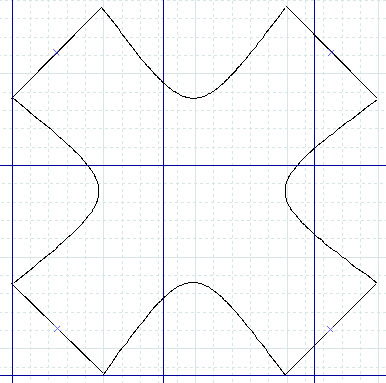
\includegraphics[width=1\linewidth]{2_2_X.png}}\\
    \end{minipage}
    \hfill
    \begin{minipage}[h]{0.47\linewidth}
        \center{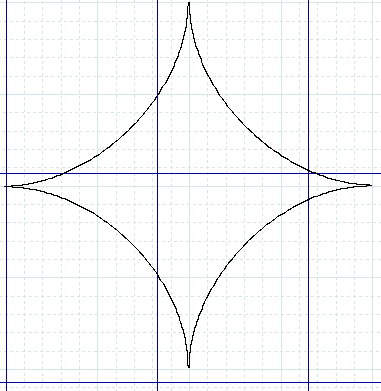
\includegraphics[width=1\linewidth]{2_3_angle_fig.png}}\\
    \end{minipage}
    \vfill
    \begin{minipage}[h]{0.47\linewidth}
        \center{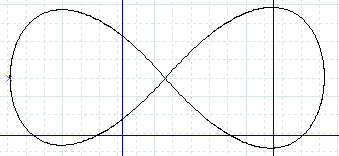
\includegraphics[width=1\linewidth]{2_1_inf.png}}
    \end{minipage}
    \hfill
    \begin{minipage}[h]{0.47\linewidth}
        \center{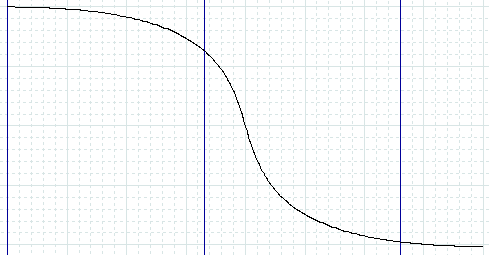
\includegraphics[width=1\linewidth]{2_4_arccot.png}}
    \end{minipage}
\end{figure}
